\subsection{Evaluation}
\label{uvm:sec:eval}

% TODO: brief intro listing the questions answered:
%   (1) Can {\uvmname} handle GPU memory oversubscription?
%   (2) How do individual design choices contribute?
%   (3) How does {\uvmname} behave on System-Allocated Memory?
%   (4) How does {\uvmname} relate to cudaMempool-based approaches?

\subsubsection{Experimental Setup}
\label{uvm:sec:eval:setup}

\paragraphb{Hardware}
We evaluate {\uvmname} on two platforms that span the
    two CPU--GPU interconnects of interest for UVM today:
    a discrete PCIe-attached system and a coherent NVLink-C2C system.
\begin{enumerate}
\item \textbf{H100-PCIe.}
    An NVIDIA H100-PCIe with $80$\,GiB of HBM,
    paired with an AMD EPYC 7413 ($24$ cores) host
    and $252$\,GiB of DDR4 system memory.
    The CPU and GPU communicate over PCIe Gen-4 ($\sim$$32$\,GB/s/dir).
    The default GPU page size is $4$\,KiB.
\item \textbf{GH200 (NVLink-C2C).}
    An NVIDIA GH200 Grace Hopper Superchip
    that integrates a $72$-core Grace CPU (Arm Neoverse-V2, single socket)
    with a Hopper GPU on a single coherent fabric.
    The Hopper GPU exposes $96$\,GiB of HBM3
    and the Grace CPU is attached to $480$\,GiB of LPDDR5X,
    all addressable from the GPU through the NVLink-C2C interconnect
    ($\sim$$450$\,GB/s/dir).
    The host runs an Arm64 Linux kernel built with $64$\,KiB base pages,
    so UVM uses $64$\,KiB managed pages on this platform---%
    a configuration we explicitly call out
    because page granularity changes the cost of UVM faults and discard.
\end{enumerate}

\paragraphb{Software}
Both platforms run the same software stack:
    PyTorch~$2.8$,
    Hugging~Face Transformers~v$4.55$,
    CUDA~$13.0$,
    and NVIDIA driver~$580.95$.
{\uvmname} is implemented as a modified \texttt{CUDACachingAllocator}
    inside this PyTorch build,
    so all baselines and {\uvmname} configurations
    share an identical Python and framework surface
    and differ only in the underlying allocator.

\paragraphb{Models and workloads}
Our primary workload is Hugging~Face causal-LM inference
    on the OPT family (OPT-$6.7$B through OPT-$175$B),
    with Qwen-$2.5$ ($7$B--$72$B) and Qwen-$1.5$ ($110$B)
    used to confirm that results generalize across model architectures.
Each request uses a context length of $2048$ tokens
    ($1920$ prompt tokens + $128$ generated tokens).
We sweep two oversubscription axes:
    (i)~\emph{batch-size sweep}---fix the model
    (OPT-$13$B as the canonical configuration)
    and grow the batch size from $4$ to $64$,
    inflating the KV-cache footprint until the working set
    no longer fits on the GPU; and
    (ii)~\emph{model-size sweep}---fix the batch size at $1$
    and grow the model footprint until the weights alone exceed device memory.

\paragraphb{Baselines}
We compare {\uvmname} against the four classes of allocators
    described in \S\ref{uvm:sec:background}:
\begin{enumerate}
\item \textbf{C1, vanilla PyTorch.}
    The stock \texttt{CUDACachingAllocator} on top of \texttt{cudaMalloc}.
    Fast when the working set fits;
    OOMs the moment it does not.
\item \textbf{A2, application-level weight offload.}
    Hugging~Face's built-in CPU offloading of model weights,
    which manually streams parameters between host and device
    around each forward pass.
\item \textbf{U0, default UVM.}
    A \texttt{CUDAPluggableAllocator} that forwards every allocation
    to \texttt{cudaMallocManaged} (first-touch placement),
    representing the naive way to use UVM in PyTorch today.
\item \textbf{U1, {\uvmname}.}
    Our full design,
    combining the UVM-aware caching allocator,
    UVM-specific active GC,
    and framework-guided eviction
    (\S\ref{uvm:sec:design:caching},~\S\ref{uvm:sec:design:discard}).
\end{enumerate}

\paragraphb{Metrics}
We report end-to-end request latency,
    decomposed where relevant into
    Time-to-First-Token (TTFT) and Inter-Token Latency (ITL).
% For ablations we additionally instrument
%     eviction traffic volume and time,
%     GPU kernel time,
%     and the number and latency of UVM page faults,
%     which lets us attribute end-to-end gains
%     to specific design decisions.

\subsubsection{Pytorch-UVM Performance}
\label{uvm:sec:eval:oversub}

% TODO: top-line result --- {\uvmname} runs to completion in
% regimes where the native allocator OOMs, while staying close
% to the in-memory baseline when not oversubscribed.

\paragraph{Concurrent requests}
\label{uvm:sec:eval:oversub:prompts}
% Fix the model size and sweep the number of concurrent prompts
% (i.e., grow the KV cache) until the workload is oversubscribed.

% --------------GH200 NVLink-C2C--------------
\begin{figure}[H]
    \centering
    \begin{subfigure}{\linewidth}
        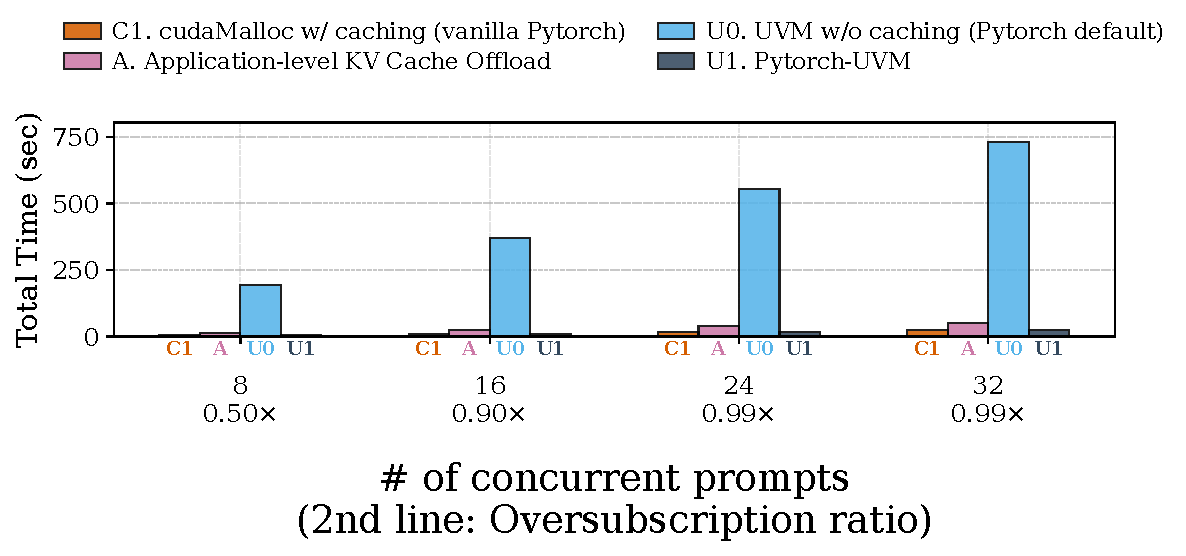
\includegraphics[width=\linewidth]{figures/eval_batch_size_gh200_small.pdf}
        \caption{Performance before oversubscription (batch size 8--32)}
        \label{uvm:fig:eval:batch_size_gh200_small}
    \end{subfigure}
    
    \begin{subfigure}{\linewidth}
        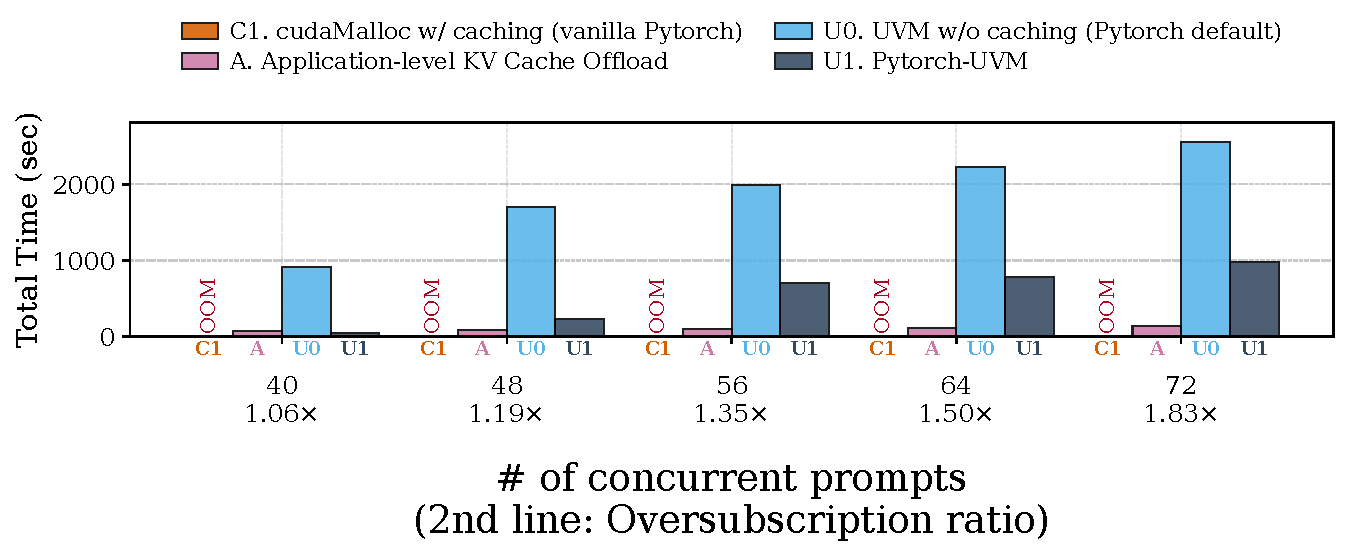
\includegraphics[width=\linewidth]{figures/eval_batch_size_gh200_large.pdf}
        \caption{Performance after oversubscription (batch size 40--72)}
        \label{uvm:fig:eval:batch_size_gh200_large}
    \end{subfigure}
    \caption{Total run time on GH200 NVLink-C2C for varying batch sizes on OPT-13B.}
    \label{uvm:fig:eval:batch_size_gh200}
\end{figure}

\paragraphb{GH200 NVLink-C2C}
Figure~\ref{uvm:fig:eval:batch_size_gh200} shows the total run time of OPT-13B on the GH200 platform as we scale the number of concurrent prompts. We split the results into two regimes: before oversubscription (batch size 8 to 32) and after oversubscription (batch size 40 to 72).

\textbf{Before oversubscription} (Figure~\ref{uvm:fig:eval:batch_size_gh200_small}), the total working set comfortably fits in the physical GPU memory. Vanilla PyTorch (C1) and {\uvmname} (U1) achieve nearly identical performance (within $5\%$ at batch size 32). In contrast, the application-level KV cache offload (A) incurs a significant overhead ($2.2\times$ slower) due to manually moving tensors between the CPU and GPU. The PyTorch default UVM (U0) performs worse by orders of magnitude ($30\times$ slower) due to the lack of user-space caching, exposing every allocation to the driver.

\textbf{After oversubscription} (Figure~\ref{uvm:fig:eval:batch_size_gh200_large}), the total working set grows to exceed the 96\,GiB HBM limit (from $1.06\times$ oversubscribed at batch size 40 up to $1.83\times$ at batch size 72). Vanilla PyTorch (C1) consistently fails with an Out-Of-Memory (OOM) error in this regime. 
{\uvmname} (U1), however, runs seamlessly, and provides a massive speedup over default UVM (U0)---for example, $19\times$ faster at batch size 40 and $2.6\times$ faster at batch size 72.

Compared to the application-level KV cache offload (A) in the oversubscribed regime, {\uvmname} (U1) is initially faster at light oversubscription ($1.38\times$ faster at batch size 40). 
However, at heavy oversubscription (batch size 48 to 72), the application-level offload outperforms {\uvmname} (U1), 
because the former refactors application code to explicitly move KV cache tensors to GPU before they are needed, 
whereas {\uvmname} relies on transparent page faults and UVM-level eviction heuristics. 
Nonetheless, {\uvmname} achieves functional oversubscription completely transparently 
without the engineering complexity of explicit KV cache management.

% --------------H100 PCIe (4\,KiB pages)--------------
\begin{figure}[H]
    \centering
    \begin{subfigure}{\linewidth}
        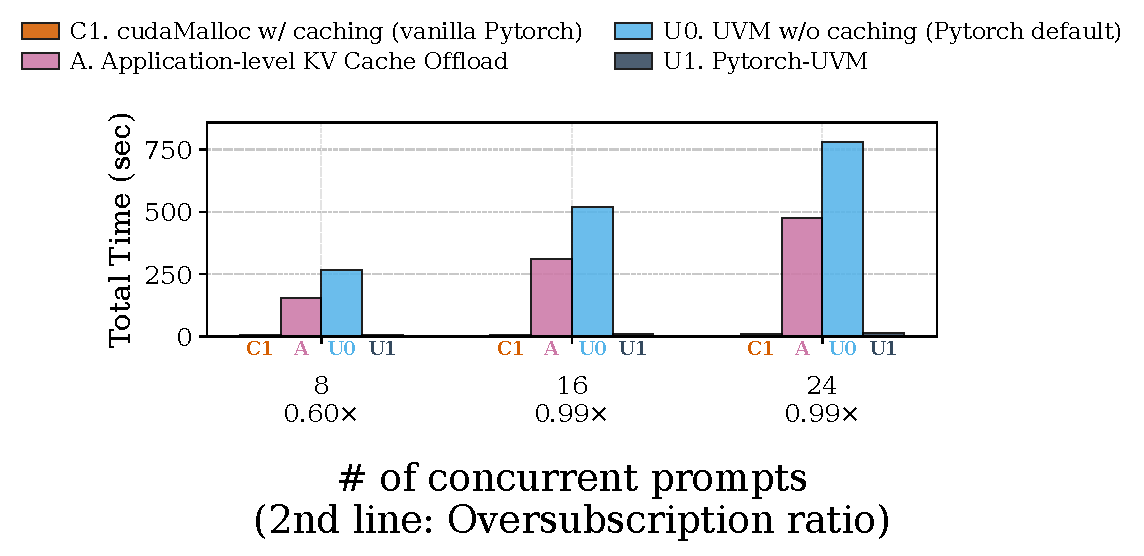
\includegraphics[width=\linewidth]{figures/eval_batch_size_h100_small.pdf}
        \caption{Performance before oversubscription (batch size 8--24)}
        \label{uvm:fig:eval:batch_size_h100_small}
    \end{subfigure}
    
    \begin{subfigure}{\linewidth}
        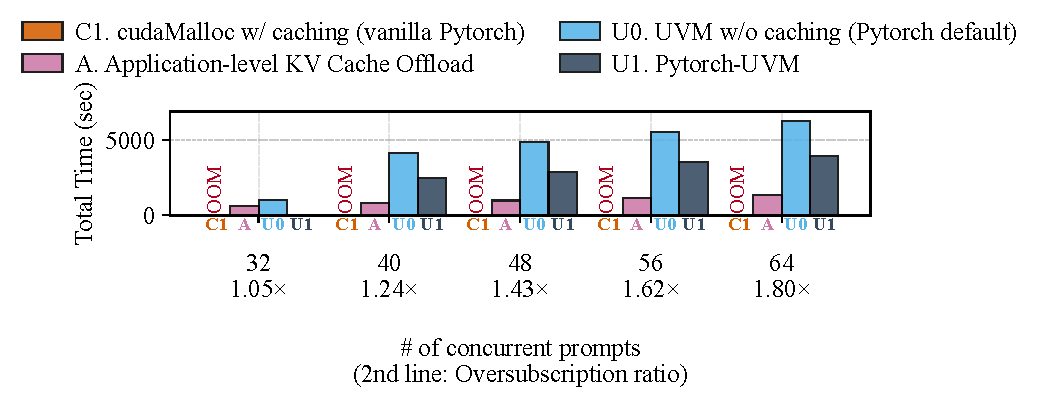
\includegraphics[width=\linewidth]{figures/eval_batch_size_h100_large.pdf}
        \caption{Performance after oversubscription (batch size 32--64)}
        \label{uvm:fig:eval:batch_size_h100_large}
    \end{subfigure}
    \caption{Total run time on H100 PCIe (4\,KiB pages) for varying batch sizes on OPT-13B.}
    \label{uvm:fig:eval:batch_size_h100}
\end{figure}

\paragraphb{H100 PCIe}
Figure~\ref{uvm:fig:eval:batch_size_h100} shows the total run time of OPT-13B on the H100 PCIe platform
    as we scale the number of concurrent prompts.
We split the results into two regimes:
    before oversubscription (batch size 8 to 24)
    and after oversubscription (batch size 32 to 64).

\textbf{Before oversubscription} (Figure~\ref{uvm:fig:eval:batch_size_h100_small}),
    the total working set fits in the 80\,GiB HBM
    (oversubscription ratio of $0.60\times$ at batch size 8 to $0.99\times$ at batch size 24).
Vanilla PyTorch (C1) and {\uvmname} (U1) achieve nearly identical performance.
In contrast, application-level KV cache offload (A) is roughly $35\times$ slower than {\uvmname},
    because every forward pass must stream the KV tensors
    over the comparatively narrow PCIe Gen-4 link.
PyTorch default UVM (U0) is even worse,
    roughly $57\times$ slower than {\uvmname},
    as it pays a UVM page-fault round-trip for every cold access
    without any user-space caching.

\textbf{After oversubscription} (Figure~\ref{uvm:fig:eval:batch_size_h100_large}),
    the total working set exceeds the 80\,GiB HBM limit
    (from $1.05\times$ oversubscribed at batch size 32
    up to $1.80\times$ at batch size 64).
Vanilla PyTorch (C1) fails with OOM across the entire range.
{\uvmname} (U1) runs to completion in every configuration
    and outperforms default UVM (U0) throughout
    (e.g., a $45\times$ speedup at batch size 32 and a $1.6\times$ speedup at batch size 64).
At very light oversubscription (batch size 32, $1.05\times$),
    {\uvmname} stays close to the in-memory baseline
    and is also more than $27\times$ faster than application-level offload.

Beyond batch size 32, however,
    the comparison with application-level offload reverses on H100 PCIe:
    A is $\sim$$3\times$ faster than {\uvmname} across batch sizes 40 to 64.
Unlike on GH200, where NVLink-C2C makes transparent UVM page faults relatively cheap,
    PCIe Gen-4's much lower bandwidth amplifies the per-fault cost,
    so the perfectly synchronous CPU--GPU streaming of application-level offload pays off
    as soon as the working set materially exceeds device memory.
{\uvmname} still delivers oversubscription transparently
    and significantly improves over default UVM,
    but on the discrete-PCIe interconnect
    there is a clear performance gap to hand-tuned application-level offload
    at heavy oversubscription.

\paragraph{Large models}
\label{uvm:sec:eval:oversub:models}
% Fix the prompt and sweep the model size (weights footprint)
% until the model alone exceeds GPU memory.

\begin{figure}[H]
    \centering
    \begin{subfigure}{\linewidth}
        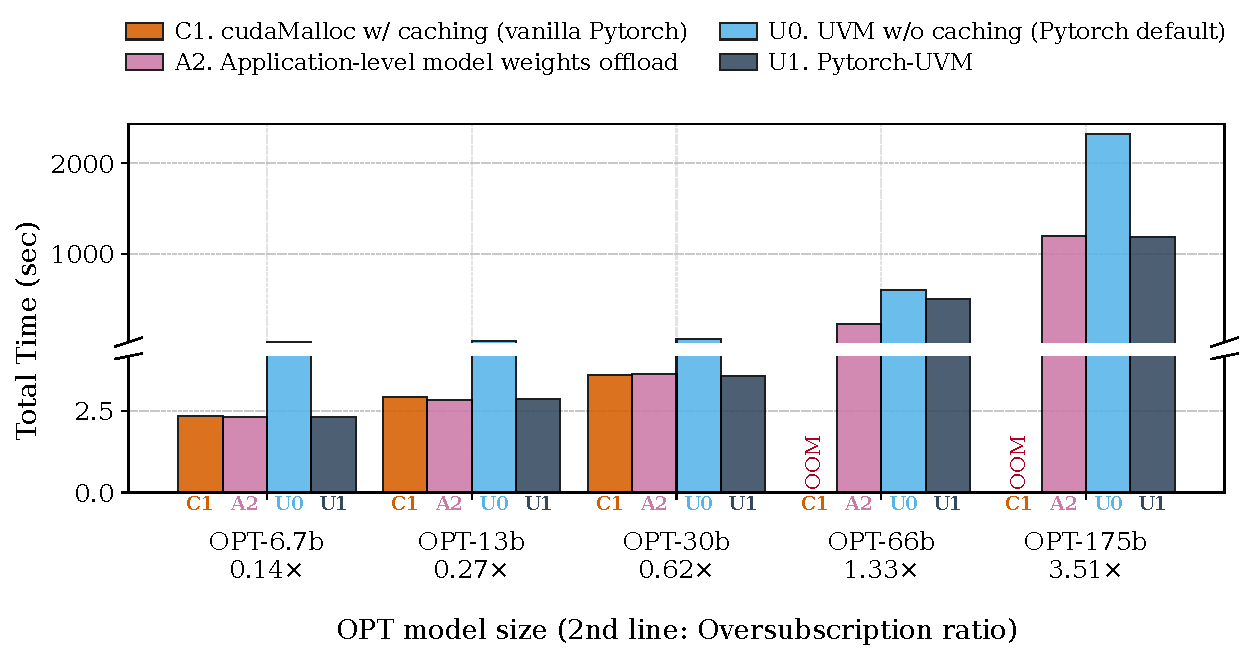
\includegraphics[width=\linewidth]{figures/total_run_time_vs_opt_model_size_on_gh200_64k_prompt1920_decode128_bsz1.pdf}
        \caption{OPT models}
        \label{uvm:fig:eval:opt_model_size}
    \end{subfigure}
    
    \begin{subfigure}{\linewidth}
        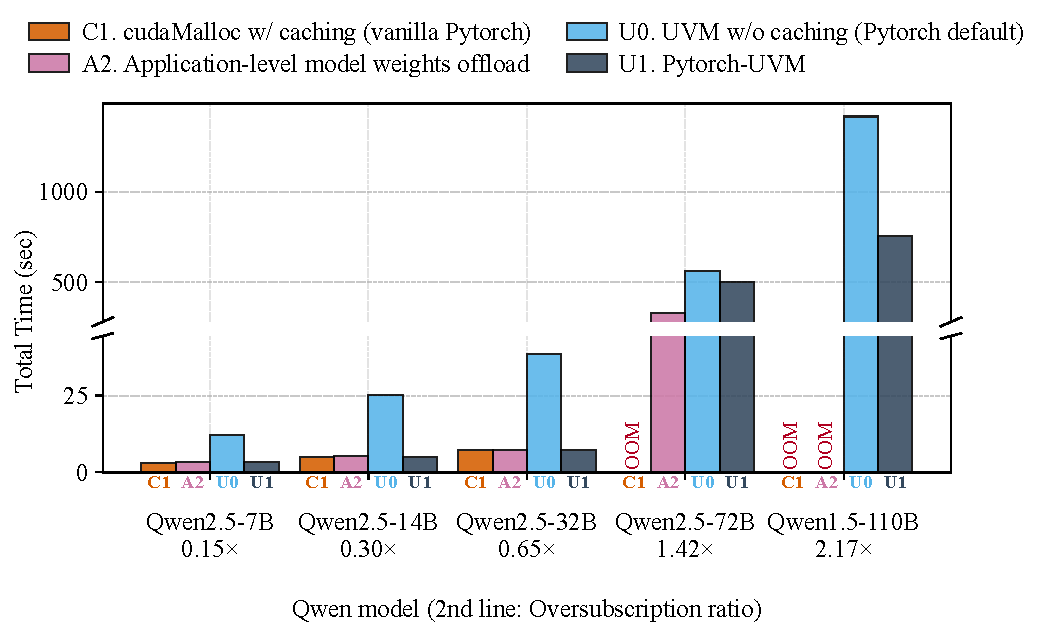
\includegraphics[width=\linewidth]{figures/total_run_time_vs_qwen_model_size_on_gh200_64k_prompt1920_decode128_bsz1.pdf}
        \caption{Qwen models}
        \label{uvm:fig:eval:qwen_model_size}
    \end{subfigure}
    \caption{Total run time on GH200 NVLink-C2C for varying model sizes.}
    \label{uvm:fig:eval:model_size_gh200}
\end{figure}

\paragraphb{GH200 NVLink-C2C}
Figure~\ref{uvm:fig:eval:model_size_gh200} shows the total run time of OPT and Qwen models
    on a GH200 system with 64\,KiB pages.
As the model size increases,
    the memory footprint eventually exceeds the physical GPU memory capacity. 

Vanilla PyTorch (C1) fails with an Out-Of-Memory (OOM) error
    on the largest models (OPT-66B, OPT-175B, Qwen2.5-72B, and Qwen1.5-110B),
    because its native allocator expects memory to be strictly device-resident.
Application-level weight offload (A2) runs all models
    by manually streaming weights between the CPU and GPU,
    avoiding OOM at the cost of application complexity;
    default UVM (U0) likewise avoids OOM by transparently spilling pages to host,
    but degrades severely under oversubscription
    due to unrestrained allocation growth and eviction thrashing.

{\uvmname} (U1) runs all models transparently.
When memory is not oversubscribed
    (e.g., OPT-6.7B--OPT-30B, Qwen2.5-7B--Qwen2.5-32B),
    it matches vanilla PyTorch (C1) and A2,
    showing that our user-space caching
    and UVM-specific active garbage collection (\S\ref{uvm:sec:design:caching})
    eliminate the overhead of managed memory in the common case.
When the GPU is oversubscribed,
    {\uvmname} outperforms default UVM (U0) by a large margin
    (e.g., $1.95\times$ on OPT-175B and $1.87\times$ on Qwen1.5-110B),
    while still matching the application-level weight-offload baseline (A2)
    without any manual changes to application code.

\begin{figure}[H]
    \centering
    \begin{subfigure}{\linewidth}
        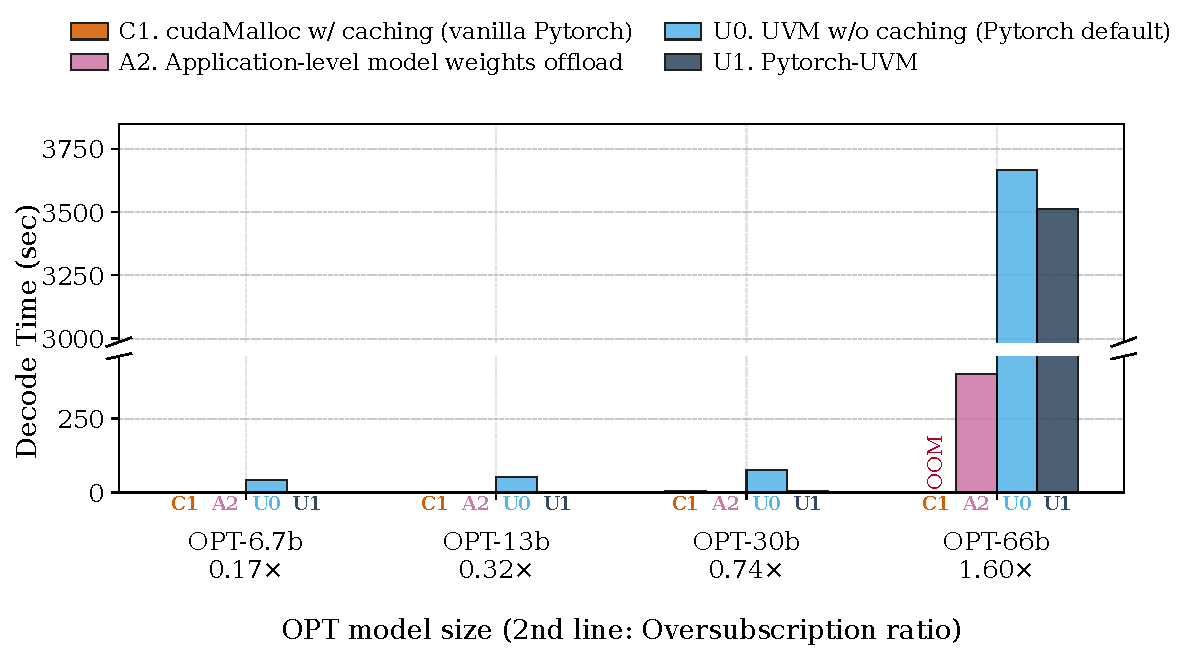
\includegraphics[width=\linewidth]{figures/decode_time_vs_opt_model_size_on_h100_64k_prompt1920_decode128_bsz1.pdf}
        \caption{OPT models (decode time)}
        \label{uvm:fig:eval:opt_model_size_h100}
    \end{subfigure}
    
    \begin{subfigure}{\linewidth}
        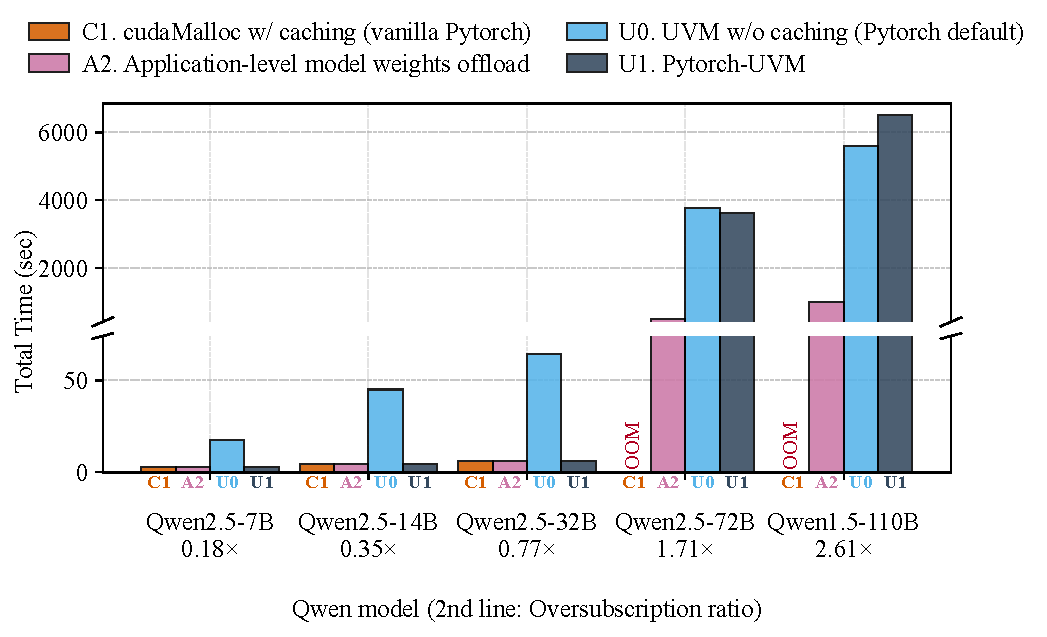
\includegraphics[width=\linewidth]{figures/total_run_time_vs_qwen_model_size_on_h100_64k_prompt1920_decode128_bsz1.pdf}
        \caption{Qwen models (total run time)}
        \label{uvm:fig:eval:qwen_model_size_h100}
    \end{subfigure}
    \caption{Run time on H100 PCIe for varying model sizes
        (1920 prompt + 128 decode tokens, batch size 1).
        OPT-175B is omitted because its weights exceed the host's 252\,GiB of system memory,
        so all UVM-based baselines fail with a host OOM
        before they can begin streaming pages to the GPU.}
    \label{uvm:fig:eval:model_size_h100}
\end{figure}

\paragraphb{H100 PCIe}
Figure~\ref{uvm:fig:eval:model_size_h100} repeats the model-size sweep on the H100 PCIe platform.
We omit OPT-175B from this sweep
    because the model's roughly $350$\,GB of fp16 weights
    exceed the host's $252$\,GiB of system memory:
    every UVM-based baseline (U0, U1, and even A2) fails with a host-side OOM
    before it can stream the first page to the GPU,
    so there is no meaningful number to report.

\textbf{Below the device-memory limit.}
For models whose weights fit in the $80$\,GiB of HBM
    (OPT-6.7B--OPT-30B and Qwen2.5-7B--Qwen2.5-32B),
    {\uvmname} (U1), vanilla PyTorch (C1),
    and application-level offload (A2) are essentially indistinguishable,
    while default UVM (U0) is roughly $10$--$20\times$ slower.
This mirrors the GH200 result and confirms that
    {\uvmname}'s caching and active GC eliminate UVM's per-allocation overhead
    on H100 PCIe just as effectively as on NVLink-C2C.

\textbf{Above the device-memory limit.}
On the largest models that still fit in host memory
    (OPT-66B, Qwen2.5-72B, Qwen1.5-110B),
    Vanilla PyTorch (C1) OOMs as expected,
    and the gap between U1 and U0 narrows or even reverses on H100:
    on OPT-66B U1 is only $\sim$$5\%$ faster than U0;
    on Qwen2.5-72B $\sim$$4\%$ faster;
    and on Qwen1.5-110B {\uvmname} is actually $\sim$$1.17\times$ slower than U0.
Application-level offload (A2) wins decisively across the board on these models,
    roughly $7$--$9\times$ faster than {\uvmname} on H100 PCIe.

This is in sharp contrast to GH200 NVLink-C2C,
    where {\uvmname} achieved $1.95\times$ and $1.87\times$ speedups over U0
    on OPT-175B and Qwen1.5-110B respectively
    (\S\ref{uvm:sec:eval:oversub:models}, GH200 paragraph).
The first-order explanation is interconnect bandwidth.
At batch size 1 the decode loop reads the model's weights once per token,
    so the achievable throughput is set by how fast pages can move from host to GPU.
NVLink-C2C provides $\sim$$450$\,GB/s/dir,
    leaving the interconnect with enough headroom that
    eliminating spurious eviction and re-fault traffic
    (the work that framework-guided eviction and the active GC do)
    translates directly into end-to-end speedup.
PCIe Gen-4 provides only $\sim$$32$\,GB/s/dir
    --- more than $10\times$ less ---
    so on H100 the link itself is the bottleneck for both U0 and U1
    in this regime,
    and the savings from smarter eviction are largely absorbed
    by the link being saturated either way.
A2's hand-tuned synchronous streaming
    keeps the PCIe link continuously busy without the per-page-fault overheads,
    which is why it dominates here.
We expect this gap to shrink on PCIe Gen-5 / NVLink-attached H100 variants
    where the bandwidth-to-compute ratio more closely resembles GH200,
    but on the discrete-PCIe-Gen-4 platform
    {\uvmname} primarily delivers oversubscription transparency
    rather than a meaningful performance edge over U0
    in the model-weights-dominated regime.

\subsubsection{Analysis of Design Choices}
\label{uvm:sec:eval:design}

% Per-design-choice ablations, isolating the contribution of
% each component of {\uvmname}.

\paragraph{Trade-off of Framework-guided Eviction with UVMDiscard}
\label{uvm:sec:eval:design:discard}

\begin{figure}[H]
    \centering
    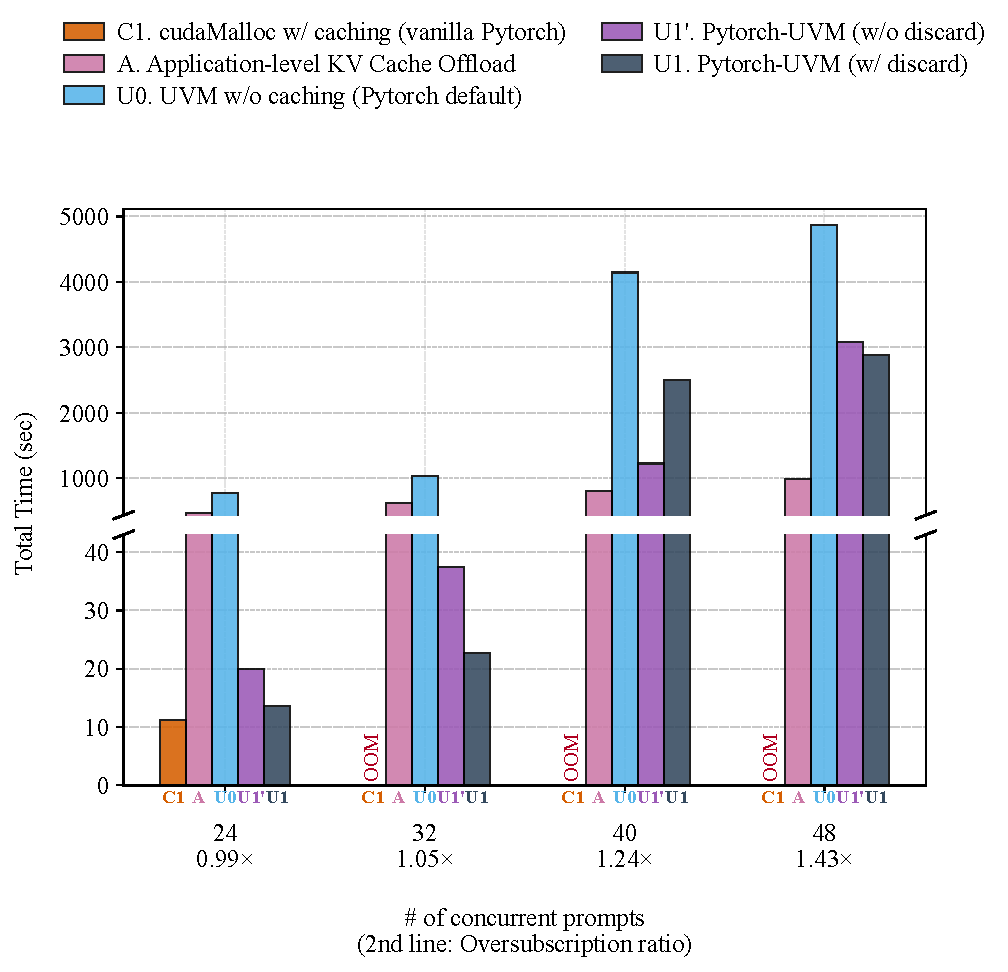
\includegraphics[width=\linewidth]{figures/eval_discard_h100.pdf}
    \caption{Effect of framework-guided eviction on H100 PCIe (4\,KiB pages):
        total run time of OPT-13B for batch sizes spanning the oversubscription transition.
        U1 enables framework-guided eviction (implemented via UVMDiscard);
        U1' keeps the rest of {\uvmname} but evicts via copy-back to host.
        Reserved / active oversubscription ratios are
        bsz=24: $0.99\times$\,/\,$0.81\times$,
        bsz=32: $1.05\times$\,/\,$0.97\times$,
        bsz=40: $1.24\times$\,/\,$1.14\times$,
        bsz=48: $1.43\times$\,/\,$1.31\times$.}
    \label{uvm:fig:eval:discard_h100}
\end{figure}

\paragraphb{H100 PCIe}
Figure~\ref{uvm:fig:eval:discard_h100} isolates the contribution of framework-guided eviction (\S\ref{uvm:sec:design:discard})
    by comparing {\uvmname} with framework-guided eviction enabled (U1)
    against an otherwise-identical configuration
    that disables it and instead evicts pages by copying them back to host (U1').
The sweep covers the oversubscription transition on H100 PCIe.
We distinguish two oversubscription ratios:
    \emph{reserved} oversubscription is the size of the allocator's reserved memory pool relative to HBM,
    while \emph{active} oversubscription is the size of the live working set
    (pages that PyTorch is actively using at any one time)
    relative to HBM.
At bsz 24--32 the workload is reserved-oversubscribed
    ($0.99\times$ and $1.05\times$)
    but \emph{active}-undersubscribed ($0.81\times$ and $0.97\times$),
    while at bsz 40--48 even the active working set exceeds HBM
    ($1.14\times$ and $1.31\times$).
Vanilla PyTorch (C1), default UVM (U0), and application-level offload (A)
    are shown for reference.

\textbf{Active oversub $<$ 1 (bsz 24, 32).}
When the actively-used pages still fit on the GPU,
    our framework-guided eviction is a decisive win:
    U1 is $1.46\times$ faster than U1' at bsz 24
    and $1.64\times$ faster at bsz 32.
The pages that get evicted in this regime are exactly the ones
    that the allocator has marked as cached/freed
    (KV blocks for completed steps, scratch buffers, etc.),
    and {\uvmname}'s allocator can tell UVM that those pages are safe to drop.
This is the design intent of \uvmname:
    information that lives in the framework---which buffers are still semantically live---%
    is normally invisible to the GPU MMU,
    and exposing it lets us avoid pure-overhead copy-backs to host.
U1' loses this information, so even when active oversub is below 1
    every eviction still pays the full PCIe round-trip,
    and the resulting end-to-end gap is roughly the volume of those wasted copies.

\textbf{Active oversub $>$ 1 (bsz 40, 48).}
Once the live working set itself exceeds HBM,
    the trend reverses or flattens:
    U1 (framework-guided eviction) is $2.04\times$ slower than U1' at bsz 40,
    and the two variants are within $7\%$ at bsz 48.
The pages that {\uvmname} now evicts are no longer dominated by safely-discardable cached blocks;
    they include genuinely live data
    that is re-touched within the same forward pass.
In this regime, framework-guided eviction provides no benefit over plain copy-back:
    the same thrashing occurs either way.
Worse, at bsz 40 discard is not merely neutral but adds overhead of its own.
When a discarded block is later reused,
    {\uvmname} prepopulates it on the GPU to avoid page faults at kernel-execution time.
At an active oversubscription ratio just above $1$ (e.g., bsz 40),
    this produces a discard-reuse ping-pong:
    a page is discarded to reclaim space
    and then almost immediately back-populated onto the GPU for its next use,
    so the bandwidth discard was meant to save is instead spent
    shuttling the same page back and forth.
% On the narrow PCIe Gen-4 link this extra re-fault cost
%     outweighs the eviction bandwidth that discard saves,
%     so U1 falls behind U1' in this regime.
Note that both variants nonetheless remain $\geq$$1.6\times$ faster than U0,
    and both are substantially slower than application-level offload (A)
    for the same reasons discussed in \S\ref{uvm:sec:eval:oversub:prompts}.

The takeaway is that framework-guided eviction pays off precisely when
    PyTorch holds framework-level information that UVM otherwise cannot see:
    namely, that some currently-resident pages are cached but inactive allocations
    rather than live data.
This is the regime where {\uvmname} stays close to the in-memory baseline,
    and our design of passing framework-level information is what lets it close the last gap to C1.
Once the active working set itself exceeds device memory
    that signal is no longer there to exploit.
    % and the cheaper option on a discrete interconnect is to keep the host-side copy.
% We revisit how to recover discard's benefit in this regime
%     when discussing access-counter-driven placement in \S\ref{uvm:sec:eval:design:counters}.
\paragraph{Trade-off of Access Counters}
\label{uvm:sec:eval:design:counters}

\begin{figure}[H]
    \centering
    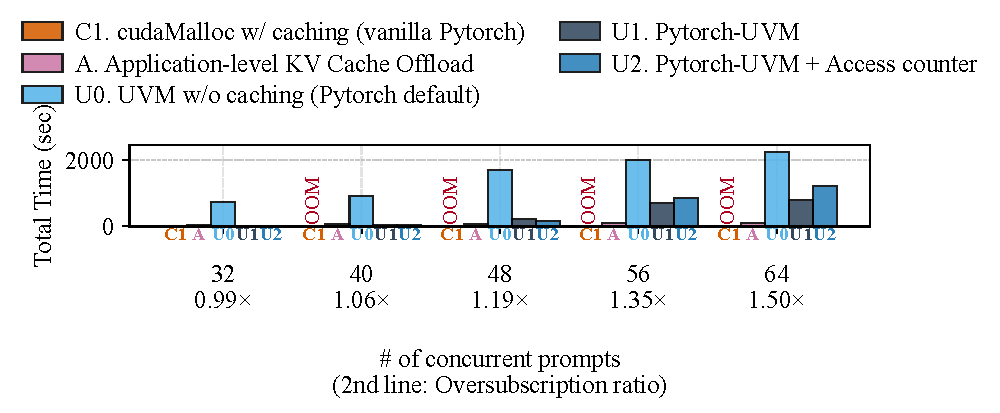
\includegraphics[width=\linewidth]{figures/eval_access_counter_gh200.pdf}
    \caption{Effect of access-counter--driven placement on GH200 NVLink-C2C:
        total run time of OPT-13B for batch sizes 32--64
        ($0.99\times$--$1.50\times$ oversubscribed).
        U1 is {\uvmname} without access counters;
        U2 enables access-counter--driven migration on top of U1.}
    \label{uvm:fig:eval:access_counter_gh200}
\end{figure}

\paragraphb{GH200 NVLink-C2C}
We restrict this ablation to GH200
    because access-counter--driven migration in the current NVIDIA driver
    is only supported for $64$\,KiB UVM-managed and system-allocated memory;
    the H100 PCIe path with $4$\,KiB pages does not expose access counters today,
    so an apples-to-apples comparison is not yet possible there.

Figure~\ref{uvm:fig:eval:access_counter_gh200} compares {\uvmname} (U1)
    against an otherwise-identical configuration that additionally enables
    access-counter--driven migration (U2),
    over batch sizes 32--64 ($0.99\times$--$1.50\times$ reserved oversubscription).
The effect of access counters is non-monotonic in oversubscription pressure
    and breaks into three regimes.

\textbf{Before oversubscription (bsz 32).}
Access counters add no measurable overhead in the unoversubscribed regime:
    U1 and U2 are within noise of each other at bsz 32,
    matching the in-memory baseline (C1).
Counter-driven migration is only triggered when pages cross the migration threshold,
    so when no pages are being faulted in cold from host
    the mechanism is effectively dormant.

\textbf{Onset of thrashing (bsz 40, 48; $1.06$--$1.19\times$).}
At light active oversubscription
    access counters mitigate thrashing:
    U2 is $1.43\times$ faster than U1.
At this point the working set just exceeds HBM,
    so a small set of hot pages is being faulted in repeatedly;
    counters quickly identify those pages
    and pin them on the GPU instead of letting them be evicted again,
    which is exactly the access pattern that the mechanism is designed for.

\textbf{Heavier thrashing (bsz 56, 64).}
As oversubscription grows further the trend reverses:
    U2 is up to $1.55\times$ \emph{slower} than U1
    at bsz 56 and 64.
Once a large fraction of the working set is hot,
    the counters cannot promote pages in time
    --- by the construction of the driver's static threshold,
    a page must be touched several times from the GPU
    before it is migrated ---
    so accesses still pay the full GPU-to-CPU round-trip,
    and the additional accounting and migration traffic
    becomes net overhead rather than net benefit.

The takeaway is that the absolute benefit of access counters
    depends sharply on the working-set profile,
    even within a single workload (OPT-13B inference) on a single platform.
The current UVM driver uses a fixed migration threshold,
    which is well-tuned for the bsz-48 regime
    but is too conservative under heavier thrashing
    and pays for itself only narrowly.
A dynamic threshold that adapts to the observed fault rate and reuse distance
    would let the mechanism remain helpful at higher oversubscription ratio.
    % without becoming a tax at high oversubscription ratio.
\paragraph{Trade-off of No migration}
\label{uvm:sec:eval:design:direct}

\begin{figure}[H]
    \centering
    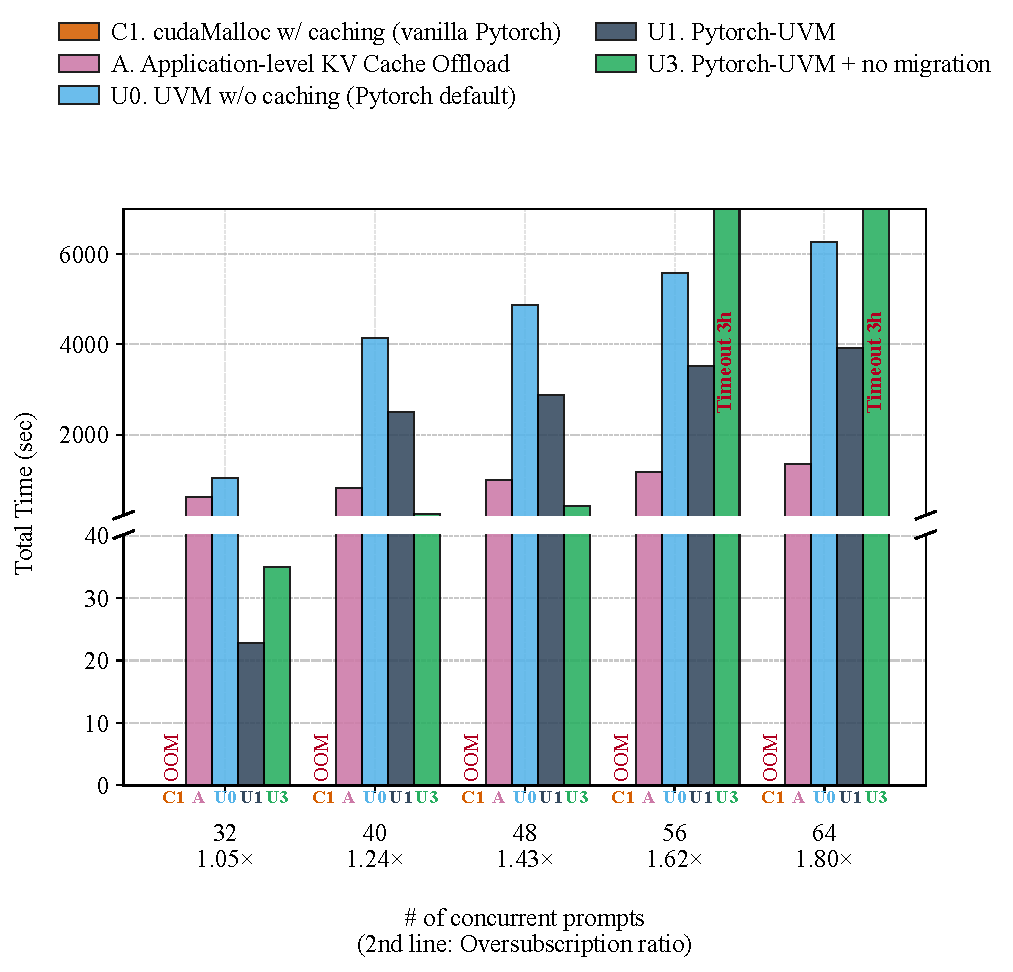
\includegraphics[width=\linewidth]{figures/eval_no_migration_h100.pdf}
    \caption{Effect of disabling migration on H100 PCIe (4\,KiB pages):
        total run time of OPT-13B for batch sizes 32--64.
        U1 is {\uvmname} with on-demand migration;
        U3 is the same configuration with migration disabled,
        so that pages are accessed in place over PCIe (zero-copy).
        Reserved / active oversubscription ratios are
        bsz=32: $1.05\times$\,/\,$0.97\times$,
        bsz=40: $1.24\times$\,/\,$1.14\times$,
        bsz=48: $1.43\times$\,/\,$1.31\times$,
        bsz=56: $1.62\times$\,/\,$1.48\times$,
        bsz=64: $1.80\times$\,/\,$1.65\times$.
        Bars at $10{,}800$\,s indicate runs that hit the 3-hour timeout.}
    \label{uvm:fig:eval:no_migration_h100}
\end{figure}

\paragraphb{H100 PCIe}
The thrashing we observed for U1 in \S\ref{uvm:sec:eval:design:discard}
    is a direct consequence of the default UVM migration policy:
    whenever the GPU touches a non-resident page,
    the driver eagerly faults it in
    and, if necessary, evicts another page to make room.
Once the active working set exceeds HBM,
    every fault-in forces a follow-up eviction,
    with too little reuse in between to amortize the PCIe round-trip.
Configuration U3 keeps the rest of {\uvmname} unchanged
    but disables on-demand migration,
    so any GPU reference to a non-resident page
    is served \emph{in place} over PCIe (zero-copy).
Figure~\ref{uvm:fig:eval:no_migration_h100} compares U1 and U3 across the oversubscription transition.
The effect breaks into three regimes.

\textbf{Active oversub $<$ 1 (bsz 32).}
When the live working set still fits on the GPU,
    disabling migration is strictly detrimental:
    U3 is $1.54\times$ slower than U1.
There is no thrashing to avoid:
    framework-guided eviction already lets the allocator keep only the live pages resident
    and silently drop cached/freed ones,
    so U1's placement is essentially optimal.
U3 just replaces each one-time page-in with a per-access PCIe round-trip,
    most visibly in prefill,
    where U3's throughput is $\sim$$2.5\times$ lower than U1's.

\textbf{Moderate oversub (bsz 40, 48).}
Once the active working set just exceeds HBM,
    disabling migration is a decisive win:
    U3 is $10.5\times$ faster than U1 at bsz 40
    and $6.94\times$ faster at bsz 48.
Here U1's eager fault-in becomes counterproductive
    --- a page is migrated in, displaces another page that is touched again shortly after,
    and the displaced page is faulted back in ---
    so most of the wall time is spent on PCIe traffic that produces no useful residency.
U3 short-circuits the cycle by leaving those pages on host,
    trading higher per-access latency for the elimination of eviction churn.

\textbf{Heavier thrashing (bsz 56, 64).}
As oversubscription grows further the working set itself grows,
    and accessing all of it over PCIe stops being viable:
    U3 fails to complete within the 3-hour timeout
    at bsz 56 and 64,
    while U1 still completes.
With $1.48\times$--$1.65\times$ active oversubscription,
    every layer streams through hundreds of MiB of weights and KV per step;
    if none of that is allowed to migrate,
    each step is bottlenecked end-to-end on a $\sim$$25$\,GB/s PCIe Gen-4 link.
U1 can at least keep some hot pages resident
    and amortize their fault-in across many accesses,
    so even with heavy fault traffic it beats raw zero-copy by more than an order of magnitude.

The takeaway is that whether migration helps or hurts
    depends on how much of the working set is hot and how fast the host link is.
On PCIe Gen-4 H100 the eager-migration default is right
    at low and very high oversubscription,
    but is exactly wrong in the moderate middle (bsz 40, 48),
    where in-place access avoids the eviction-and-refault cycle
    and recovers up to $10.5\times$.
We expect this picture to shift on GH200,
    whose $\sim$$450$\,GB/s/dir NVLink-C2C link makes in-place access far cheaper
    and should extend the regime where U3 beats U1;
    a full GH200 sweep is left to future work.

\subsubsection{System-Allocated Memory (SAM)}
\label{uvm:sec:eval:sam}

\begin{figure}[H]
    \centering
    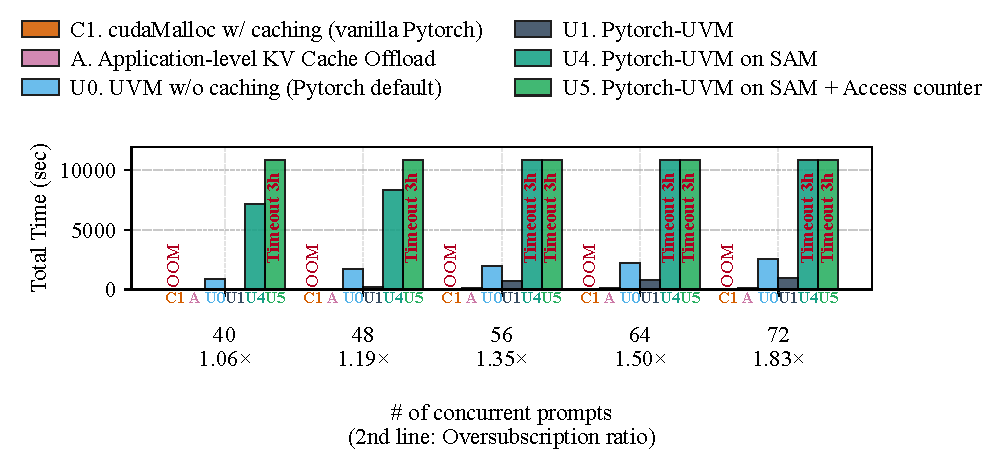
\includegraphics[width=\linewidth]{figures/eval_sam_gh200.pdf}
    \caption{Performance of {\uvmname} on System-Allocated Memory (SAM)
        on GH200 NVLink-C2C, OPT-13B, batch sizes $8$--$72$.
        U4 uses ordinary \texttt{malloc} memory accessed via ATS.
        U5 adds access-counter--based migration to the SAM path.
        Baselines C1, A, U0, and U1 (managed memory) are shown for reference.}
    \label{uvm:fig:eval:sam_gh200}
\end{figure}

\paragraph{ATS-Based SAM (GH200, 64\,KiB)}
\label{uvm:sec:eval:sam:ats}

We evaluate {\uvmname} on System-Allocated Memory (SAM) on the GH200 NVLink-C2C system,
    where the GPU accesses ordinary \texttt{malloc}'d host pages
    via Address Translation Services (ATS).
\figurename~\ref{uvm:fig:eval:sam_gh200} compares the SAM-backed PyTorch-UVM (U4)
    against the \texttt{cudaMallocManaged}-backed version (U1)
    and other baselines.
When memory is not oversubscribed (batch sizes $8$--$32$),
    the SAM path (U4) performs identically to the managed-memory path (U1),
    matching vanilla PyTorch (C1) and delivering $\sim$$2500$--$3000$ e2e tokens/s.
This confirms that ATS-based SAM introduces no overhead
    for resident working sets.

However, as soon as the active working set exceeds GPU memory (batch size $40$ and beyond),
    the SAM path's performance collapses.
At batch size $40$ (active oversubscription $1.06\times$),
    U4 is $149\times$ slower than U1.
At batch sizes $56$ and above, U4 times out after 3 hours ($>$$10{,}800$\,s).
Adding access-counter--based migration to the SAM path (U5)
    fails to rescue performance;
    it times out at batch size $40$ and beyond.

The severe degradation under oversubscription stems from
    the lack of UVM-aware optimizations on the SAM path.
Unlike \texttt{cudaMallocManaged},
    SAM allocations currently do not support UVMDiscard,
and migration bandwidth is also limited on ATS-based SAM.
% TODO: Optimize the SAM path by exposing discard and prefetch equivalents
% for ATS-backed memory, or by tuning the OS-level page reclamation policies
% to better align with PyTorch's caching allocator.

\paragraph{HMM-Based SAM (H100)}
\label{uvm:sec:eval:sam:hmm}
We port {\uvmname} to the HMM-based SAM path on H100 PCIe,
    which lets the GPU access ordinary \texttt{malloc}'d host pages
    via Linux's Heterogeneous Memory Management
    rather than going through \texttt{cudaMallocManaged}.
On the same OPT-13B / 16-concurrent-prompt configuration
    used in \S\ref{uvm:sec:eval:oversub:prompts},
    the HMM-backed run takes \emph{over 3 hours}
    to complete a single end-to-end inference
    --- more than $1200\times$ slower than {\uvmname}
    on top of \texttt{cudaMallocManaged}.

The order-of-magnitude gap reflects the cost of HMM's per-fault path on H100 PCIe.
Every device access to a host page is resolved through
    a Linux MMU-notifier callback into the NVIDIA driver,
    which migrates the page over PCIe one fault at a time
    and offers no equivalent of the \texttt{cudaMemAdvise} /
    prefetch / discard hints
    that {\uvmname}'s allocator uses to amortize and avoid faults
    on the \texttt{cudaMallocManaged} path.
As a result, the HMM path on H100 today is functional
    but not yet competitive with managed-memory UVM,
    and we report this configuration primarily to characterize
    the gap between the two SAM mechanisms
    rather than as a performance recommendation.
% TODO: HMM path on H100 --- once the driver exposes the equivalent advise/prefetch/discard
% hooks, rerun and compare against the cudaMallocManaged numbers above.

\subsubsection{Comparison with cudaMempool}
\label{uvm:sec:eval:mempool}

\begin{figure}[H]
    \centering
    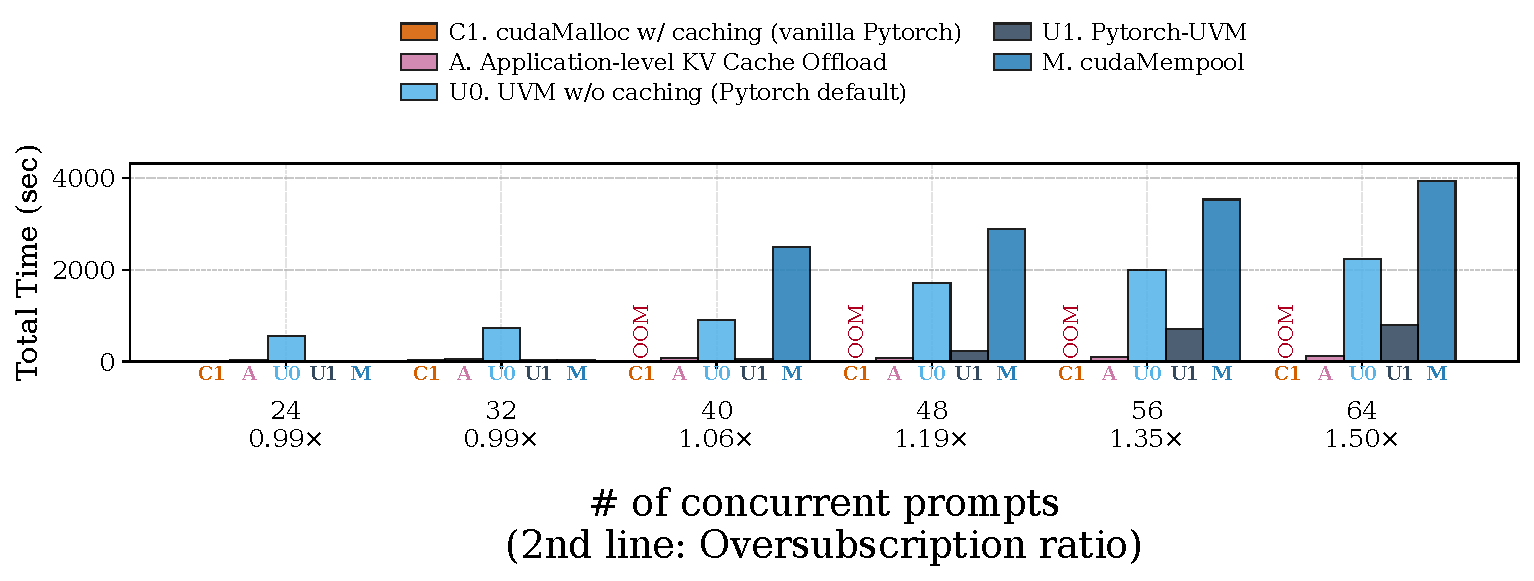
\includegraphics[width=\linewidth]{figures/eval_mempool_gh200.pdf}
    \caption{Comparison of {\uvmname} (U1) and a cudaMempool-based allocator (M)
        on GH200 NVLink-C2C, OPT-13B, batch sizes $24$--$64$
        ($0.99\times$--$1.50\times$ reserved oversubscription).
        Both allocators sit on top of \texttt{cudaMallocManaged};
        baselines C1, A, and U0 are shown for reference.
        At bsz $72$ ($1.83\times$) cudaMempool fails with a host-side OOM
        and is therefore omitted from the rightmost point.}
    \label{uvm:fig:eval:mempool_gh200}
\end{figure}

CUDA's mempool API is the closest in-tree alternative to {\uvmname}'s caching layer
    --- runtime-level allocator caching, applicable to any CUDA application,
    and backable by either \texttt{cudaMalloc} or \texttt{cudaMallocManaged}.
We compare against the most-favorable configuration
    (a \texttt{cudaMallocManaged}-backed mempool)
    on GH200 NVLink-C2C using the same OPT-13B sweep
    as in \S\ref{uvm:sec:eval:oversub:prompts}.

Before oversubscription (bsz 24, 32),
    {\uvmname} (U1) and cudaMempool (M) are essentially equivalent
    (within noise at bsz 24 and 32).
Once the workload becomes oversubscribed, however, the two diverge sharply:
    at bsz 40 ($1.06\times$ oversubscribed) cudaMempool is $52\times$ slower than {\uvmname},
    the gap stays large through bsz 64 ($5.0\times$),
    and at bsz 72 ($1.83\times$) cudaMempool exhausts host memory and OOMs entirely
    while {\uvmname} still completes.
The cause is that cudaMempool retains pooled allocations indefinitely
    and never returns the underlying UVM-managed pages to the driver,
    so its reserved working set grows monotonically
    and the driver is forced to handle a much larger working set than the real active footprint.
    The host-OOM at bsz 72 is the same failure mode pushed to its limit.

This is not a fundamental limitation of the mempool design.
We believe that a mempool implementation with {\uvmname}-style active garbage collection could recover most of {\uvmname}'s performance
    while still being a general-purpose allocator for any CUDA application.
% The cudaMempool API already exposes a release threshold and explicit trim hooks
%     (\texttt{cudaMemPoolAttrReleaseThreshold}, \texttt{cudaMemPoolTrimTo}),
%     and extending those to actively release UVM-managed pages
%     when the pool grows beyond a target footprint
%     would let a UVM-aware cudaMempool recover most of {\uvmname}'s behavior
%     while keeping the API's broader applicability.
